\documentclass{standalone}
\usepackage{tikz}
\usepackage{amsmath}

\begin{document}

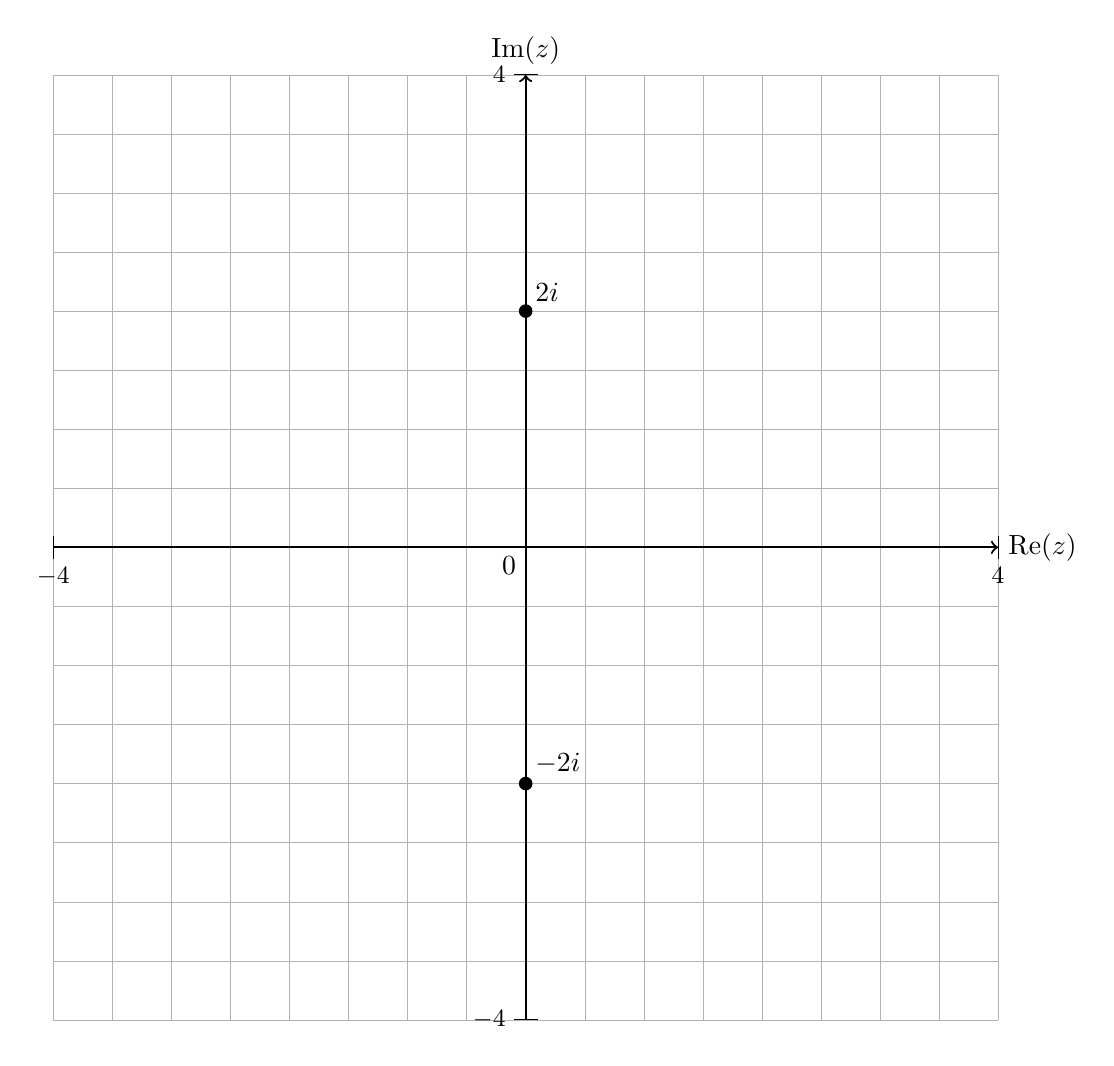
\begin{tikzpicture}[scale=1.5]
    
    % Center of the circle
    \def\xmin{-4}
    \def\xmax{4}
    \def\ymin{-4}
    \def\ymax{4}
    \def\dx{.5}
    \def\dy{.5}
    \def\xminb{\xmin-\dx}
    \def\xmaxb{\xmax+\dx}
    \def\yminb{\ymin-\dy}
    \def\ymaxb{\ymax+\dy}
    \coordinate (z1) at (0., 2.);
    \coordinate (z2) at (0., -2.);

    % Draw grid
    \draw[step=0.5, gray!60, ultra thin] (\xmin, \ymin) grid (\xmax, \ymax); % Visible grid with lighter color
    
    % Axes
    \draw[->, thick] (\xmin, 0) -- (\xmax, 0) node[right] {$\text{Re}(z)$};
    \draw[->, thick] (0, \ymin) -- (0, \ymax) node[above] {$\text{Im}(z)$};

    % Axis ticks
    \foreach \x in {\xmin, \xmax}
        \draw (\x, -0.1) -- (\x, 0.1) node[below=8pt] {\small $\x$};
    \foreach \y in {\ymin, \ymax}
        \draw (-0.1, \y) -- (0.1, \y) node[left=8pt] {\small $\y$};

    % Labels for axes
    \node[below left] at (0, 0) {$0$};

    % Zeros
    \filldraw[black] (z1) circle (1.5pt) node[above right] {$ 2i$};
    \filldraw[black] (z2) circle (1.5pt) node[above right] {$-2i$};

\end{tikzpicture}

\end{document}

